\documentclass[a4paper, 12pt]{article}
\usepackage[utf8]{inputenc}
\usepackage[russian]{babel}
\usepackage{amsmath}
\usepackage{graphicx}
\usepackage{hyperref}

\title{TEncDM: Понимание свойств диффузионной модели в пространстве кодировок языковых моделей}
\author{Лапиков Владислав}
\date{}

\begin{document}

\maketitle

\begin{abstract}
Представленная работа описывает Text Encoding Diffusion Model (TEncDM) — новаторский подход к моделированию текста с помощью диффузионной модели, работающей в пространстве кодировок языковой модели. В отличие от традиционных методов, основанных на эмбеддингах, TEncDM использует кодировки, которые содержат больше контекстной информации и улучшают качество предсказаний модели. Кроме того, в модели используется трансформерный декодер, специально разработанный для учета контекста при предсказании токенов, а также самоконтроль, что повышает точность генерации текста. Экспериментальные результаты на задачах перефразирования, суммаризации и упрощения текста подтверждают превосходство TEncDM над традиционными неавторегрессивными диффузионными моделями.
\end{abstract}

\section{Введение}
Авторегрессивные модели, такие как GPT-4 \cite{gpt4} и Llama 3 \cite{llama3}, демонстрируют высокое качество в задаче генерации текста. Они создают текст, проходя последовательно по каждому токену, что делает их подход надежным и естественным для создания длинных связных текстов. Однако эти модели имеют два значительных недостатка. Во-первых, они не могут корректировать ошибки, допущенные на ранних этапах генерации. Поскольку авторегрессивные модели генерируют текст слева направо, любая ошибка, допущенная на начальных шагах, будет "разрастаться", искажая весь последующий текст. Во-вторых, авторегрессивный подход требует обработки каждого токена по отдельности, что замедляет процесс генерации, особенно на длинных последовательностях.

Диффузионные модели, активно развивающиеся в таких областях, как генерация изображений, аудио и видео, предлагают альтернативный метод. В диффузионных моделях процесс генерации происходит параллельно, что позволяет генерировать всю последовательность токенов одновременно. Это делает модель более гибкой и позволяет обрабатывать и корректировать любые части текста в процессе генерации, что ускоряет работу. Кроме того, диффузионные модели позволяют сократить количество необходимых вычислительных операций путем дистилляции, что также сокращает время генерации текста.

Существует множество подходов к адаптации диффузионных моделей для текстовой генерации, от замены гауссовского шума на категориальный до обучения на небольших латентных представлениях текста. Однако еще не найден оптимальный подход, который позволил бы эффективно моделировать текст с учетом особенностей его структуры и содержания. В данной работе исследуется возможность обучения диффузионной модели в латентном пространстве контекстуальных кодировок, предоставляемых языковыми моделями. Мы выделили и проанализировали влияние декодера, шумового расписания и метода самоконтроля на качество генерации текста, что позволило сформулировать основные рекомендации по разработке диффузионных моделей для текстовой генерации.

\section{Постановка задачи и принципы диффузионного моделирования}
Задача генерации текста заключается в построении текста, который удовлетворяет заданному условию, например, теме или стилю. Диффузионное моделирование предполагает преобразование случайного шума в структурированный текст. Для обучения модели требуется "прямой процесс диффузии", в котором шум постепенно добавляется к латентному представлению текста, и "обратный процесс", в ходе которого модель обучается восстанавливать исходный текст на основе зашумленного представления. При этом диффузионная модель должна учитывать контекст и структуру текста на всех этапах денойзинга, чтобы восстановить полноценную текстовую последовательность.

\section{Методология}
Методология TEncDM включает несколько ключевых компонентов, которые позволяют повысить качество генерации текста за счет учета контекста и контроля шума на каждом этапе денойзинга.

\begin{figure}[t]
\begin{center}
\centerline{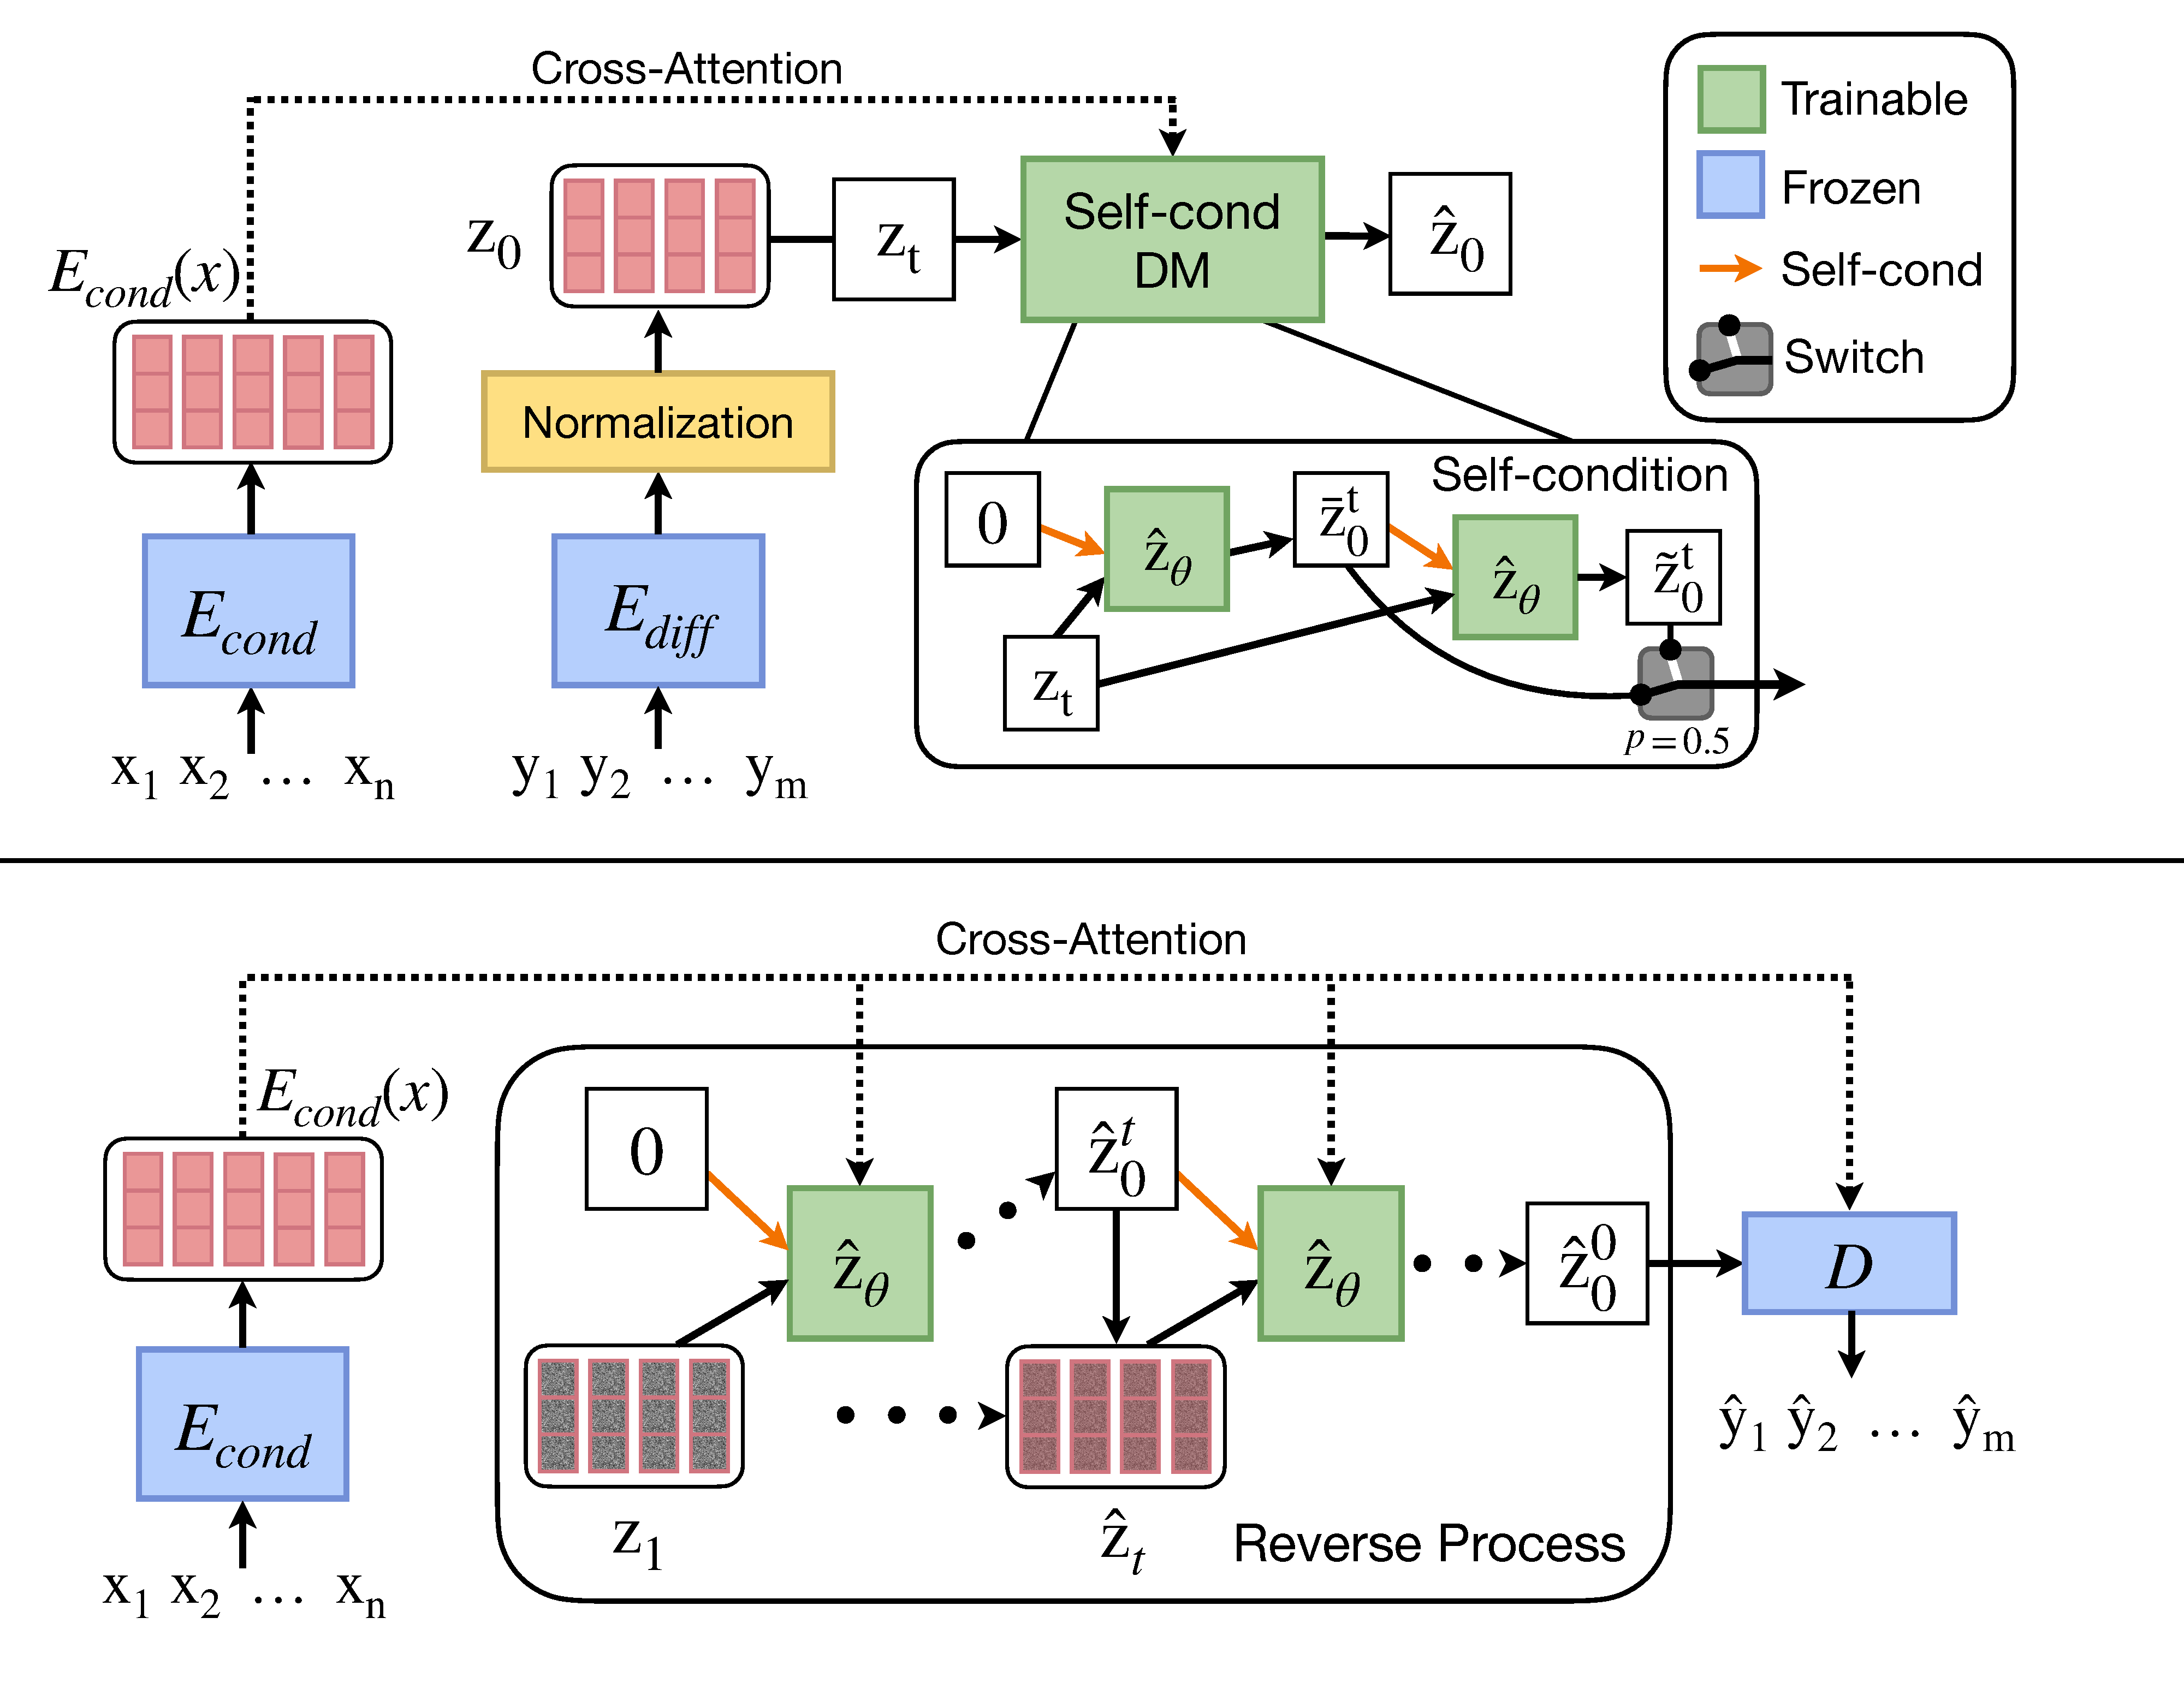
\includegraphics[width=\columnwidth]{images/framework.pdf}}
\caption{Обзор фреймворка для условной генерации. Вверху - процесс обучения, внизу - процесс генерации.}
\label{fig::model_pipeline}
\end{center}
\end{figure}

\subsection{Кодировщик}
TEncDM использует предварительно обученную трансформерную модель для преобразования текста в латентное пространство кодировок, которое содержит контекстную информацию. В отличие от эмбеддингов, которые представляют токены фиксированными значениями, кодировки адаптируются к контексту, в котором находятся, что позволяет модели лучше понимать смысл текста. Кодировщик обрабатывает каждое предложение, преобразуя его в последовательность латентных переменных, выровненных по длине для корректной обработки в модели.

\subsection{Диффузионная модель}
Диффузионная модель TEncDM построена на базе трансформера с 12 слоями и обучается восстанавливать исходные латенты из зашумленных версий. Для этого используется шумовое расписание, в котором интенсивность шума контролируется параметром, что позволяет задать сложность восстановления на каждом шаге. Чем выше шум, тем сложнее диффузионной модели восстановить исходный текст, но это способствует более устойчивому обучению модели. Таким образом, контролируемое добавление шума помогает улучшить точность генерации текста.

\subsection{Декодер}
После этапа денойзинга декодер преобразует восстановленные латенты в текст. В TEncDM применяется трансформерный декодер, который учитывает контекст для каждого токена, что улучшает качество предсказаний. Декодер обучается независимо от диффузионной модели, чтобы его работа не зависела от ошибок, допущенных на предыдущих шагах. Таким образом, даже если диффузионная модель допускает неточность при восстановлении латентов, декодер способен скорректировать результат, улучшив итоговое качество текста.

\subsection{Самоконтроль}
Введение самоконтроля позволяет диффузионной модели повышать точность предсказаний на каждом шаге, ориентируясь на собственные предыдущие предсказания. В модели реализовано два сценария самоконтроля: с нулевым значением (для случаев, когда предыдущая информация отсутствует) и с учетом данных из предыдущего шага. Эксперимент показал, что самоконтроль позволяет модели сократить количество шагов денойзинга, что ускоряет процесс генерации.


\section{Обзор литературы и открытых источников по теме генерации текстов с помощью диффузионных моделей}

С момента появления диффузионных моделей и подтверждения их успешности для генерации изображений было предпринято немало попыток адаптации их для генерации текста. Все предоженные подходы можно разделить на две категории: дискретные диффузионные модели (Discrete Diffusion Models) и непрерывные диффузионные модели (Continuous Diffusion Models). Дискретные модели эксплуатируют дискретность текстовых данных и зашумляют их с помощью шума из категориального распределения. Непрерывные модели сперва переводят текст в непрерывный вид, например, с помощью замены токенов на их векторные представления, а после этого зашумляют данные стандартным гауссовским шумом. 

На данный момент нельзя сказать однозначно, какое из этих направлений является более успешным. Обе области активно развиваются и каждый год пополняются новыми подходами. Далее мы рассмотрим подробнее методы каждой из этих категорий, чтобы сформировать представление о состоянии области.

В данном разеделе описан обзор и выводы в соответствии с анализом источников с 32 по 51, указанных в том числе в списке использованных источников.


\subsection{Discrete Diffusion Models}

Процесс зашумление – главное отличие между дискретными и непрерывными диффузионными моделями. В дискретных моделях каждый токен представляется в виде one-hot векторов (1 соответствует индексу токена, на всех остальных позициях стоят 0). Тогда, один шаг удаления информации записывается по формуле
\begin{align}
q(x_t | x_{t-1}) = \text{Cat}(x_t; p = x_{t-1}Q_t),
\end{align}
где $x_t$ – набор one-hot векторов, соответствующих одному тексту на шаге зашумления  $t$, а $Q_t$ – стохастическая матрица перехода, переводящаяя каждый токен в вероятности перехода в другой токен. Для выбора матрицы $Q_t$ существует несколько подходов. Два основные из них подробно разобраны в статье \cite{d3pm}:

1. \textbf{Равномерное распределение:} $Q_t = \alpha_{t|t-1} \boldsymbol{I} + \sigma_{t|t-1} / K$ \\

2. \textbf{Поглощающее распределение:} $[Q_t]_{i j}=\left\{\begin{array}{lll}
1 & \text { if } & i=j=m \\
\alpha_{t|t-1} & \text { if } & i=j \neq m \\
\sigma_{t|t-1} & \text { if } & j=m, i \neq m
\end{array}\right.
$, \\
где $m$ – индекс токена маски [MASK]. Таким образом, каждый токен маскируется независимо с некоторой вероятностью.

Равномерное распределение применяется в работах \cite{mtd, sedd}, а поглощающее – в \cite{sedd, diffusionbert, diffusionnat, mdlm, simplifiedmaskeddiffusion}.

Помимо способа удаления информации, методы дискретной диффузии различаются по предсказываемой сущности. В то время как \cite{d3pm, diffusionbert, mtd, mdlm} предсказывают $x_0$, обучая модель с помощью кросс-энтропии, \cite{concretescorematching} показывает, что вместо этого можно предсказывать вектор из отношения плотностей всех токенов к плотности токена на текущем шаге, $s(x, t) = \bigg[\frac{p_t(y)}{p_t(x)}\bigg]_{y \neq x}$. В \cite{sedd} эта идея развивается и предлагается новая функция ошибки на основе дивергенции Брегмана, улучшающая качество генерации текстов.


\subsection{Continuous Diffusion Models}

Непрерывные диффузионные модели повторяют идею диффузионных моделей, применяемых для изображений и аудио. В них объект зашумляется с помощью вливания в него гауссовского шума.
\begin{align}
    q(x_t | x_s) = \mathcal{N}(x_t; \alpha_{t|s} x_{s}, \sigma_{t|s}^2 I)
\end{align}

Для текста в числовом формате чаще всего используются векторные представления токенов фиксированной длины \cite{diffusionlm, diffuseq, yuan2022seqdiffseq, lin2023genie, planner, dinoiser, difformer}. Однако иногда модель обучают на симплексе \cite{han2023ssdlmsemiautoregressivesimplexbaseddiffusion, mahabadi2024tesstexttotextselfconditionedsimplex}, представляя каждый токен в виде вектора ${+k, -k}^{|V|}$, где $+k$ стоит на месте индекса токена, а на всех остальных позициях стоит $-k$.

\subsubsection{Расписание зашумления}
Еще одной важной особенностью непрерывной диффузии является выбор расписания зашумления. В статьях \cite{diffusionlm, difformer, dinoiser} показано, что для текстовых диффузионных моделей требуется добавлять больше шума на ранних итерациях зашумления, чем для картиночных моделей. Данный феномен связан с дискретной сущностью текстов – векторные представления хорошо разделяют токены из-за проклятья размерности. Поэтому при добавлении небольшого количества шума каждый токен можно без труда восстановить и задача диффузионной модели становится слишком простой.

\subsubsection{Self-conditioning}
Также для непрерывных диффузионных моделей был предложен подход self-conditioning \cite{analogbits, sed}. Он модифицирует процесс генерации, добавляя в модель ее предсказание на предыдущем шаге в качестве условия $\hat{x}^{t-1}_0 = p_{\theta}(x_{t-1} | x_t, \hat{x}^t_0)$. Несмотря на то, что такая модификация позволяет значительно улучшить качество генерации модели, почему именно это происходит – открытый вопрос. Для добавления self-conditioning процесс обучения тоже видоизменяется: с вероятностью 50\% модель получает на вход пустое условие, $p_{\theta}(x_{t-1} | x_t, 0)$, и с вероятностью 50\% свое предсказание для объекта $x_t$, $p_{\theta}(x_{t-1} | x_t, \hat{x}^{t}_0)$. Данная схема необходима для того, чтобы было возможно сделать первое предсказание на шаге $T$, когда никаких предсказаний модель еще не совершала.

\subsubsection{Декодирование текста}
В то время как самым распространенным способом декодирования текста является округление каждого сгенерированного вектора к токену с ближайшим векторным представлением \cite{diffusionlm, diffuseq}, были предложены и другие методы.
В работах \cite{planner, ld4lg} применяется авторегрессионная модель для генерации текста, которая получает на вход сгенерированные векторы в качестве условия.



\section{Экспериментальный анализ}
Для проверки эффективности TEncDM были проведены эксперименты на задачах условной генерации текста, включая перефразирование, суммаризацию и упрощение текста. Были использованы датасеты QQP \cite{qqp} (вопросы-перефразирования), XSum \cite{xsum} (экстремальная суммаризация) и Wiki-Auto \cite{wiki_auto} (упрощение текста). Модель TEncDM оценивалась на основе следующих метрик:

\begin{itemize}
    \item \textbf{Perplexity} — показатель, который измеряет логарифмическое среднее расстояние между вероятностью предсказания модели и реальными данными. Низкий уровень Perplexity указывает на высокую точность генерации.
    \item \textbf{MAUVE} — метрика, оценивающая близость распределений сгенерированного и референтного текста. MAUVE измеряет, насколько тексты, сгенерированные моделью, похожи на реальные тексты, что позволяет оценить реалистичность и связность.
    \item \textbf{Дивергенция} — метрика, которая измеряет разнообразие текстов, предотвращая дублирование и стандартизацию.
    \item \textbf{Меморизация} — метрика, которая измеряет, насколько модель запоминает данные из обучающего набора, что позволяет предотвратить чрезмерное повторение.
\end{itemize}

\subsection{Результаты экспериментов}

\begin{table}
% \setlength{\tabcolsep}{3pt}
\centering
\begin{tabular}{l|llll}
\hline
\multicolumn{1}{l|}{\textbf{Encoder}}
    & \multicolumn{1}{c}{\textbf{ppl} $\downarrow$} 
    & \multicolumn{1}{c}{\textbf{mem} $\downarrow$}
    & \multicolumn{1}{c}{\textbf{div} $\uparrow$}
    & \multicolumn{1}{c}{\textbf{mauve} $\uparrow$}\\
\hline
\multicolumn{5}{c}{\textbf{ROCStories}} \\
\hline
BERT emb & $48.9_{.36}$ & $.371_{.003}$ & $.324_{.002}$ & $.600_{.016}$ \\
BERT & $29.1_{.89}$ & ${.453}_{.003}$ & ${.295}_{.002}$ & $\textbf{.762}_{.043}$ \\
RoBERTa & $\textbf{28.3}_{.33}$ & ${.443}_{.003}$ & ${.302}_{.002}$ & ${.647}_{.019}$\\
T5 & ${31.3}_{.54}$ & $.427_{.003}$ & $.312_{.004}$ & $.706_{.024}$ \\
BART & $34.1_{.52}$ & $.441_{.006}$ & $.299_{.005}$ & $.705_{.030}$\\
\hline
Source text & $21.7$ & $.365$ & $.403$ & $.876$ \\
\hline
\multicolumn{5}{c}{\textbf{Wikipedia}} \\
\hline
BERT emb & $156.1_{1.8}$ & $.263_{.004}$ & $.517_{.002}$ & $.378_{.055}$ \\
BERT & $\textbf{104.4}_{2.1}$ & $.286_{.002}$ & $.504_{.003}$ & $\textbf{.874}_{.011}$ \\
\hline
Source text & $37.3$ & $.122$ & $.615$ & $.957$ \\
\hline
\end{tabular}
\caption{Сравнение энкодеров}
\label{tab::encoders}
\end{table}

\begin{table}
% \setlength{\tabcolsep}{3pt}
\centering
% \resizebox{0.49\textwidth}{!}{
\begin{tabular}{l|cccc}
\hline
\textbf{Decoder} & \textbf{ppl} $\downarrow$ & \textbf{mem} $\downarrow$ & \textbf{div} $\uparrow$ & \textbf{mauve} $\uparrow$ \\
\hline
\multicolumn{5}{c}{\textbf{ROCStories}} \\
\hline
MLP & $39.7_{3.38}$ & $.444_{.002}$ & $.297_{.004}$ & $.716_{.074}$ \\
\; + $Cor(z_0)$ & $31.2_{.33}$ & $.448_{.002}$ & $.293_{.003}$ & $.739_{.051}$ \\
Transformer & $34.2_{.29}$ & $.445_{.001}$ & $.295_{.003}$ & $.714_{.037}$ \\
\; + $Cor(z_0)$ & $\textbf{29.1}_{.89}$ & ${.453}_{.003}$ & ${.295}_{.002}$ & $\textbf{.762}_{.043}$ \\
\hline
\multicolumn{5}{c}{\textbf{Wikipedia}} \\
\hline
Transformer & $180.6_{3.2}$ & $.261_{.001}$ & $.511_{.001}$ & $.526_{.025}$ \\
\; + $Cor(z_0)$ & $\textbf{104.4}_{2.1}$ & $.286_{.002}$ & $.504_{.003}$ & $\textbf{.874}_{.011}$ \\
\hline
\end{tabular}
% }
\caption{Сравнение декодеров}
\label{tab::decoders}
\end{table}

Результаты экспериментов показали, что модель TEncDM превосходит другие существующие подходы в генерации текста по всем основным метрикам. Например, на задаче перефразирования модель показала значительное преимущество перед конкурентами, демонстрируя более точные перефразы при сохранении смысла. На задаче суммаризации модель смогла достичь высоких результатов, генерируя лаконичные и точные резюме. В задаче упрощения текста TEncDM также показала себя лучше других методов, успешно передавая основные мысли сложных текстов в простой форме.

Влияние отдельных компонентов на качество генерации

\textbf{Кодировщик и декодер}. Исследования показали, что использование кодировок вместо эмбеддингов позволяет модели учитывать больше контекста, а продвинутый декодер способен значительно улучшить качество текстов за счет адаптации к особенностям латентного пространства.

\textbf{Самоконтроль}. Анализ показал, что метод самоконтроля увеличивает точность предсказаний модели, особенно при генерации длинных текстов, когда важно учесть каждый шаг для сохранения связности.

\textbf{Шумовое расписание}. Контроль интенсивности шума на каждом этапе улучшил процесс обучения модели и позволил улучшить качество предсказаний, что особенно важно для обработки текстов с неоднородной структурой.



\section{Разработка стратегии увеличения большой языковой диффузионной модели на задаче генерации текста порядка 100 млн. параметров до 1 миллиарда параметров}
\subsection{Описание задачи}

Данный отчет описывает стратегию масштабирования диффузионной языковой модели генерации текста с порядка 100 млн. параметров до 1 миллиарда параметров. В ходе выполнения были рассмотрены различные подходы, проведены эксперименты с масштабированием различных частей модели (энкодера и диффузионной части), а также изучены особенности использования претрейна для предотвращения переобучения. В основе работы лежат результаты исследований и референсные данные по уже известным моделям, таким как BERT \cite{devlin2019bertpretrainingdeepbidirectional}, RoBERTa \cite{liu2019robertarobustlyoptimizedbert} и GPT-Neo \cite{kashyap2023gptneocommonsensereasoning}.

\subsection{Цели разработки алгоритма}

\begin{itemize}
    \item Разработать стратегию увеличения числа параметров модели до 1 миллиарда, не ухудшая ее качество и устойчивость.
    \item Протестировать поведение моделей с различным количеством параметров при решении задач генерации текста.
    \item Определить ключевые параметры, которые необходимо оптимизировать для успешного масштабирования.
\end{itemize}

\subsection{Методы и материалы}

\subsubsection{Исходные данные}
Для разработки и масштабирования диффузионной модели были использованы следующие компоненты:

\begin{itemize}
    \item Открытые модели вроде GPT-Neo.
    \item \textbf{Таблицы параметров}: Для сравнения были взяты размеры различных моделей, таких как BERT (108M и 334M параметров) и XLM-RoBERTa (278M, 560M и 43GB). Это помогло ориентироваться на размеры моделей и задавать параметры масштабирования диффузионной модели.
\end{itemize}

\subsubsection{Параметры моделей}
В рамках стратегии масштабирования был установлен ряд базовых параметров, таких как количество слоев ($n_{layers}$), размер модели ($d_{model}$), количество голов ($n_{head}$), размер головы ($d_{head}$) и другие. Это позволило формализовать размеры диффузионных моделей, которые использовались в экспериментах. Примерная структура моделей до и после масштабирования:

\begin{table}[h!]
\caption{Структура моделей до и после масштабирования}
\centering
\begin{tabular}{|c|c|c|c|c|c|c|}
\hline
\textbf{Diffusion} & \textbf{Параметры модели} & $n_{layers}$ & $d_{model}$ & $n_{head}$ & $d_{head}$ & \textbf{Эндодер} \\ \hline
small & 158M & 12 & 768 & 12 & 64 & bert-base \\ \hline
medium & 352M & 24 & 768 & 16 & 64 & bert-base \\ \hline
large & 1B & 32 & 1024 & 24 & 64 & bert-large \\ \hline
\end{tabular}
\end{table}

\subsection{Эксперимент 1: Генерация текста без претрейна}

\subsubsection{Описание}
Первый эксперимент был проведен с целью понять, как больший размер модели влияет на производительность без использования предварительного обучения (pretrain). Модели различного масштаба (small, medium) обучались на задачах генерации текста с прямым использованием тестовых данных.

\subsubsection{Результаты}

\begin{table}[h!]
\caption{Результаты первого эксперимента}
\centering
\begin{tabular}{|c|c|c|c|}
\hline
\textbf{Метрика (QQP)} & small & medium-352M & medium-366M \\ \hline
BLEU ↑ & 0.317 & 0.320 & 0.315 \\ \hline
PPL ↓ & 61.3 & 60.9 & 64.0 \\ \hline
\end{tabular}
\end{table}

Результаты показали незначительное улучшение качества при увеличении параметров модели до 352M, однако при дальнейшем увеличении до 366M наблюдалось переобучение. Большая модель показала относительно худшие результаты, несмотря на увеличение числа параметров.

\textbf{Вывод}: Для успешного масштабирования необходимо использовать претрейн, так как без него модели с большим количеством параметров склонны к переобучению и не демонстрируют значительного прироста качества.

\subsection{Эксперимент 2: Масштабирование на WikiPedia}

\subsubsection{Описание}
Данный эксперимент был направлен на увеличение модели до большего объема и масштабирование на задаче безусловной генерации текста (например, написание статей на основе данных из Википедии). В этом эксперименте мы проводили несколько циклов обучения с различными конфигурациями модели (small, medium, large).

\subsubsection{Результаты}

Также были проанализированы графики зависимости метрик от количества шагов обучения, что позволило определить оптимальный момент для остановки обучения во избежание переобучения.

\begin{table}[h!]
\caption{Результаты второго эксперимента}
\centering
\begin{tabular}{|c|c|c|c|c|c|}
\hline
\textbf{Diffusion} & \textbf{Параметры} & PPL ↓ & Mauve ↑ & Div ↑ & Mem ↓ \\ \hline
small (129M) & base & $77.06$ & $0.941$ & $0.556$ & $0.273$ \\ \hline
medium (276M) & base & $67.40$ & $0.947$ & $0.564$ & $0.282$ \\ \hline
large (493M) & base & $67.90$ & $0.936$ & $0.560$ & $0.277$ \\ \hline
\end{tabular}
\end{table}


\textbf{Вывод}: Увеличение количества параметров модели до уровня medium и large показало улучшение метрик качества (например, уменьшение PPL и увеличение Mauve).

\subsection{Эксперимент 3: Масштабирование на Fineweb}

\subsubsection{Описание}
В этом эксперименте были предприняты попытки увеличить модель до 1B параметров с акцентом на увеличение диффузионной части модели, так как это показало лучшие результаты в предыдущем эксперименте. Были увеличены как энкодер, так и основная диффузионная часть модели. Пропорционально увеличивалось количество слоев и количество голов внимания (head).

\begin{table}[h!]
\caption{Параметры диффузионной модели для эксперимента 3}
\centering
\begin{tabular}{|c|c|c|c|c|c|}
\hline
\textbf{Diffusion} & \textbf{Параметры модели} & $n_{layers}$ & $d_{model}$ & $n_{head}$ & $d_{head}$ \\ \hline
small & 150M & 12 & 768 & 12 & 64 \\ \hline
XL & 1B & 48 & 768 & 24 & 128 \\ \hline
\end{tabular}
\end{table}

\subsubsection{Результаты}

\begin{table}[h!]
\caption{Результаты увеличения диффузионной модели}
\centering
\begin{tabular}{|c|c|c|c|}
\hline
\textbf{Diffusion} & PPL ↓ & Mauve ↑ & Div ↑ \\ \hline
small & 64.5 & 0.886 & 0.528 \\ \hline
XL & 46.5 & 0.912 & 0.338 \\ \hline
\end{tabular}
\end{table}

Результаты показывают, что при увеличении модели до уровня XL качество текстов заметно улучшилось, однако снизилось разнообразие (Div).

\subsubsection{Увеличение энкодера}
Для того чтобы оставить количество параметров диффузионной части модели примерно на том же уровне, были добавлены два слоя проектора. Первый слой преобразует входной вектор размерности 1024 в вектор 768, второй слой преобразует выходной вектор из размерности 768 в 1024. Остальная часть модели (трансформерные слои) осталась неизменной.

\begin{table}[h!]
\caption{Результаты увеличения энкодера}
\centering
\begin{tabular}{|c|c|c|c|}
\hline
\textbf{Encoder} & PPL ↓ & Mauve ↑ & Div ↑ \\ \hline
base & \textbf{64.5} & 0.886 & 0.528 \\ \hline
large & 118.3 & 0.887 & 0.578 \\ \hline
\end{tabular}
\end{table}

Результаты показывают, что перплексия (PPL) увеличилась вдвое, хотя остальные метрики (Mauve и Div) остались практически теми же. Это говорит о том, что тексты, генерируемые моделью, усложнились, но прироста качества не было.

\textbf{Вывод}: Применение претрейна на Википедии выявило ограниченность размера этого датасета, что сдерживает дальнейшее улучшение модели. Fineweb как более крупный датасет дает лучшие результаты при масштабировании, и эксперименты показывают, что увеличение диффузионной модели лучше сказывается на метриках, чем увеличение энкодера.


\subsection{Перспективы и ограничения}
Несмотря на высокие результаты, TEncDM имеет ряд ограничений. В частности, процесс генерации замедляется для длинных текстов, так как размерность латентного пространства возрастает. В будущем возможно создание автоэнкодера, который позволит сжимать латенты, улучшая производительность модели. Кроме того, разные задачи требуют настройки параметров модели, что предполагает необходимость в проведении дополнительных исследований для нахождения оптимальных значений для каждого типа задач.

\section{Заключение}
TEncDM демонстрирует высокие результаты в задачах генерации текста, превосходя классические диффузионные и авторегрессивные модели. Работа показала, что переход от эмбеддингов к контекстуальным кодировкам улучшает качество предсказаний и способствует созданию более натуральных текстов. Предложенная модель успешно справляется с различными задачами на реальных данных, показывая универсальность и точность. В дальнейшем планируется улучшить производительность модели за счет уменьшения латентного пространства и оптимизации параметров для различных задач.

\bibliographystyle{plain}
\bibliography{references}

\end{document}
